
\documentclass[border=8pt, multi, tikz]{standalone}

\usepackage{import}
\subimport{./tex/}{init}

\usepackage{tikz}
\usetikzlibrary{quotes,arrows.meta}
\usetikzlibrary{positioning}
\usetikzlibrary{3d}
\usetikzlibrary{shapes.misc}

%Define the colors for different blocks
\definecolor{genericconvdark}{RGB}{255,193,98}
\definecolor{genericconv}{RGB}{252,210,147}
\definecolor{genericconvlight}{RGB}{253,226,184}

\definecolor{depthwisedark}{RGB}{94,238,118}
\definecolor{depthwise}{RGB}{131,249,151}
\definecolor{depthwiselight}{RGB}{171,255,185}

\definecolor{pointwisedark}{RGB}{255,193,98}
\definecolor{pointwise}{RGB}{252,210,147}
\definecolor{pointwiselight}{RGB}{253,226,184}

\definecolor{upconvdark}{RGB}{211, 104, 250}
\definecolor{upconv}{RGB}{215, 131, 246}
\definecolor{upconvlight}{RGB}{227, 163, 250}


% Connection style and colors for different operations
\definecolor{genericconvopcolor}{RGB}{253,226,184}
\newcommand{\genericconvop}{\tikz \draw[-Stealth,line width =1mm,draw=genericconvopcolor] (-0.3,0) -- ++(0.3,0);}

\definecolor{pointwiseopcolor}{RGB}{11, 191, 131}
\newcommand{\pointwiseop}{\tikz \draw[-Stealth,line width =1mm,draw=pointwiseopcolor] (-0.3,0) -- ++(0.3,0);}

\definecolor{depthwiseopcolor}{RGB}{94, 134, 247}
\newcommand{\depthwiseop}{\tikz \draw[-Stealth,line width =1mm,draw=depthwiseopcolor] (-0.3,0) -- ++(0.3,0);}

\definecolor{upconvopcolor}{RGB}{247, 99, 99}
\newcommand{\upconvop}{\tikz \draw[-Stealth,line width =1mm,draw=upconvopcolor] (-0.3,0) -- ++(0.3,0);}

\definecolor{depthwisepoolopcolor}{RGB}{94, 134, 247}
\newcommand{\depthwisepoolop}{\tikz \draw[-Stealth,line width =1mm,draw=depthwisepoolopcolor] (-0.3,0) -- ++(0.3,0);}

\definecolor{pointwisepoolopcolor}{RGB}{94, 134, 247}
\newcommand{\pointwisepoolop}{\tikz \draw[-Stealth,line width =1mm,draw=pointwisepoolopcolor] (-0.3,0) -- ++(0.3,0);}

\definecolor{convpoolopcolor}{RGB}{94, 134, 247}
\newcommand{\convpoolop}{\tikz \draw[-Stealth,line width =1mm,draw=convpoolopcolor] (-0.3,0) -- ++(0.3,0);}

\begin{document}
\begin{tikzpicture}

\tikzstyle{connection}=[ultra thick,every node/.style={sloped,allow upside down},opacity=0.7]

\tikzset{cross/.style={cross out, draw=black, minimum size=2*(#1-\pgflinewidth), inner sep=0pt, outer sep=0pt},
%default radius will be 1pt.
cross/.default={1pt}}
    

\node[canvas is zy plane at x=0] (in.jpeg) at (0,0,0)
{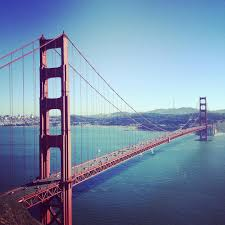
\includegraphics[width=180pt, height=180pt]{in.jpeg}};

\draw [connection] (0,0,0) -- node { \genericconvop} (2,0,0);

\pic[shift={(2,0,0)}] at (0,0,0)
	{ Box={ name=gconv11,caption= ,xlabel={ { "", } }, ylabel = , zlabel = ,
	fillface=genericconvdark,
	fillfront=genericconvlight,
	fill=genericconv, height=32,width=1,depth=32 } };

\draw [connection] (gconv11-east) -- node { \pointwiseop} (4,0,0);

\pic[shift={(4,0,0)}] at (0,0,0)
	{ Box={ name=gpointconv12,caption= ,xlabel={ { "", } }, ylabel = , zlabel = ,
	fillface=pointwisedark,
	fillfront=pointwiselight,
	fill=pointwise, height=16,width=1,depth=16 } };

\draw [connection] (gpointconv12-east) -- node { \pointwiseop} (6,0,0);

\pic[shift={(6,0,0)}] at (0,0,0)
	{ Box={ name=gconv21,caption= ,xlabel={ { "", } }, ylabel = , zlabel = ,
	fillface=pointwisedark,
	fillfront=pointwiselight,
	fill=pointwise, height=16,width=2,depth=16 } };

\draw [connection] (gconv21-east) -- node { \pointwiseop} (8,0,0);

\pic[shift={(8,0,0)}] at (0,0,0)
	{ Box={ name=gpointconv22,caption= ,xlabel={ { "", } }, ylabel = , zlabel = ,
	fillface=pointwisedark,
	fillfront=pointwiselight,
	fill=pointwise, height=8,width=2,depth=8 } };

\draw [connection] (gpointconv22-east) -- node { \pointwiseop} (10,0,0);

\pic[shift={(10,0,0)}] at (0,0,0)
	{ Box={ name=gconv31,caption= ,xlabel={ { "", } }, ylabel = , zlabel = ,
	fillface=pointwisedark,
	fillfront=pointwiselight,
	fill=pointwise, height=8,width=4,depth=8 } };

\draw [connection] (gconv31-east) -- node { \pointwiseop} (12,0,0);

\pic[shift={(12,0,0)}] at (0,0,0)
	{ Box={ name=gpointconv32,caption= ,xlabel={ { "", } }, ylabel = , zlabel = ,
	fillface=pointwisedark,
	fillfront=pointwiselight,
	fill=pointwise, height=4,width=6,depth=4 } };

\draw [connection] (gpointconv32-east) -- node { \pointwiseop} (14.3,0,0);

\pic[shift={(14.3,0,0)}] at (0,0,0)
	{ Box={ name=gconv41,caption= ,xlabel={ { "", } }, ylabel = , zlabel = ,
	fillface=pointwisedark,
	fillfront=pointwiselight,
	fill=pointwise, height=4,width=6,depth=4 } };

\draw [connection] (gconv41-east) -- node { \pointwiseop} (16.8,0,0);

\pic[shift={(16.8,0,0)}] at (0,0,0)
	{ Box={ name=gpointconv42,caption= ,xlabel={ { "", } }, ylabel = , zlabel = ,
	fillface=pointwisedark,
	fillfront=pointwiselight,
	fill=pointwise, height=2,width=8,depth=2 } };

\draw [connection] (gpointconv42-east) -- node { \pointwiseop} (19.1,0,0);

\pic[shift={(19.1,0,0)}] at (0,0,0)
	{ Box={ name=gconv52,caption= ,xlabel={ { "", } }, ylabel = , zlabel = ,
	fillface=pointwisedark,
	fillfront=pointwiselight,
	fill=pointwise, height=1,width=8,depth=1 } };

\draw [connection] (gconv52-east) -- node { \upconvop} (21.900000000000002,0,0);

\pic[shift={(21.900000000000002,0,0)}] at (0,0,0)
	{ Box={ name=gconv62,caption= ,xlabel={ { "", } }, ylabel = , zlabel = ,
	fillface=upconvdark,
	fillfront=upconvlight,
	fill=upconv, height=2,width=8,depth=2 } };

\draw [connection] (gconv62-east) -- node { \upconvop} (25.1,0,0);

\pic[shift={(25.1,0,0)}] at (0,0,0)
	{ Box={ name=gconv72,caption= ,xlabel={ { "", } }, ylabel = , zlabel = ,
	fillface=upconvdark,
	fillfront=upconvlight,
	fill=upconv, height=4,width=6,depth=4 } };

\draw [connection] (gconv72-east) -- node { \upconvop} (27.900000000000002,0,0);

\pic[shift={(27.900000000000002,0,0)}] at (0,0,0)
	{ Box={ name=gconv82,caption= ,xlabel={ { "", } }, ylabel = , zlabel = ,
	fillface=upconvdark,
	fillfront=upconvlight,
	fill=upconv, height=8,width=4,depth=8 } };

\draw [connection] (gconv82-east) -- node { \upconvop} (30.700000000000003,0,0);

\pic[shift={(30.700000000000003,0,0)}] at (0,0,0)
	{ Box={ name=gconv92,caption= ,xlabel={ { "", } }, ylabel = , zlabel = ,
	fillface=upconvdark,
	fillfront=upconvlight,
	fill=upconv, height=16,width=2,depth=16 } };

\draw [connection] (gconv92-east) -- node { \genericconvop} (33.2,0,0);

\pic[shift={(33.2,0,0)}] at (0,0,0)
	{ Box={ name=gconv10,caption= ,xlabel={ { "", } }, ylabel = , zlabel = ,
	fillface=genericconvdark,
	fillfront=genericconvlight,
	fill=genericconv, height=32,width=1,depth=32 } };

\draw [connection] (gconv10-east) -- node { \genericconvop} (34.7,0,0);

\node[canvas is zy plane at x=0] (out.jpeg) at (34.7,0,0)
{
\includegraphics[width=180pt, height=180pt]{out.jpeg}};

\draw [connection] (14.3,0,0) -- node { \depthwiseop} (14.3,0,6);

\draw [connection] (14.3,0,6) -- node { \depthwiseop} (16.3,0,6);

\pic[shift={(16.3,0,6)}] at (0,0,0)
	{ RightBandedBox={ name=residualdepth1,caption= ,xlabel={ { "", } }, ylabel = , zlabel = ,
	fillface=depthwisedark,
	fillfront=depthwiselight,
	bandfill=depthwise,
	fill=depthwise, height=4,width=8,depth=4 } };

\draw [connection] (residualdepth1-east) -- node { \depthwiseop} (23.900000000000002,0,6);

\draw [connection] (23.900000000000002,0,6) -- node { \depthwiseop} (23.900000000000002,0,0);

\draw (23.900000000000002,0,0) circle (5pt);\draw (23.900000000000002,0,0) node[cross=3pt,rotate=45,red]{};

\draw [connection] (10,0,0) -- node { \depthwiseop} (10,0,10);

\draw [connection] (10,0,10) -- node { \depthwiseop} (15,0,10);

\pic[shift={(15,0,10)}] at (0,0,0)
	{ RightBandedBox={ name=residualdepth1,caption= ,xlabel={ { "", } }, ylabel = , zlabel = ,
	fillface=depthwisedark,
	fillfront=depthwiselight,
	bandfill=depthwise,
	fill=depthwise, height=8,width=4,depth=8 } };

\draw [connection] (residualdepth1-east) -- node { \depthwiseop} (26.6,0,10);

\draw [connection] (26.6,0,10) -- node { \depthwiseop} (26.6,0,0);

\draw (26.6,0,0) circle (5pt);\draw (26.6,0,0) node[cross=3pt,rotate=45,red]{};

\draw [connection] (6,0,0) -- node { \depthwiseop} (6,0,15);

\draw [connection] (6,0,15) -- node { \depthwiseop} (11,0,15);

\pic[shift={(11,0,15)}] at (0,0,0)
	{ RightBandedBox={ name=residualdepth1,caption= ,xlabel={ { "", } }, ylabel = , zlabel = ,
	fillface=depthwisedark,
	fillfront=depthwiselight,
	bandfill=depthwise,
	fill=depthwise, height=16,width=2,depth=16 } };

\draw [connection] (residualdepth1-east) -- node { \depthwiseop} (29.200000000000003,0,15);

\draw [connection] (29.200000000000003,0,15) -- node { \depthwiseop} (29.200000000000003,0,0);

\draw (29.200000000000003,0,0) circle (5pt);\draw (29.200000000000003,0,0) node[cross=3pt,rotate=45,red]{};

\draw [connection] (2,0,0) -- node { \depthwiseop} (2,0,25);

\draw [connection] (2,0,25) -- node { \depthwiseop} (7,0,25);

\pic[shift={(7,0,25)}] at (0,0,0)
	{ RightBandedBox={ name=residualdepth1,caption= ,xlabel={ { "", } }, ylabel = , zlabel = ,
	fillface=depthwisedark,
	fillfront=depthwiselight,
	bandfill=depthwise,
	fill=depthwise, height=32,width=1,depth=32 } };

\draw [connection] (residualdepth1-east) -- node { \depthwiseop} (31.700000000000003,0,25);

\draw [connection] (31.700000000000003,0,25) -- node { \depthwiseop} (31.700000000000003,0,0);

\draw (31.700000000000003,0,0) circle (5pt);\draw (31.700000000000003,0,0) node[cross=3pt,rotate=45,red]{};


\end{tikzpicture}
\end{document}
    